\documentclass[acmsmall,screen]{acmart}
  \citestyle{acmauthoryear}

  % \documentclass[acmsmall,10pt]{acmart}\settopmatter{printfolios=true} % ,review
% \citestyle{acmauthoryear}
\usepackage{subcaption}
\usepackage[T1]{fontenc}
\usepackage[utf8]{inputenc}
\usepackage[british]{babel}
\usepackage{xspace, listings, lstcustom, wrapfig, graphicx, enumerate}
\usepackage{paralist}
\usepackage{color, colortbl, relsize}
\usepackage{rotating}
\usepackage{pifont}
\usepackage{multirow}
\usepackage{soul}
\usepackage{tcolorbox}
\usepackage[scaled=.9, light]{zlmtt}
\usepackage{siunitx}
\usepackage{setspace}

   \newcommand{\ttt}{\prg{true}}
\newcommand{\ff}{\prg{false}}
\newcommand{\unkn}{\prg{b???}}
\newcommand{\bv}{\prg{bval}}

\newcommand{\sdparagraph}[1]{{\vspace{.3cm} \noindent \textit{#1}\ }}

\newcommand{\prg}[1]{{\mbox{\tt{#1}}}}

\newcommand{\m}{\prg{m}}
 \newcommand{\f}{\prg{f}}
  \newcommand{\e}{\prg{e}}
 \renewcommand{\c}{\prg{C}}
 \renewcommand{\v}{\prg{v}}
  \newcommand{\x}{\prg{x}}
  \newcommand{\p}{\prg{p}}
   \newcommand{\y}{\prg{y}}
      \newcommand{\uu}{\prg{u}}
  %  \newcommand{\z}{\prg{z}}
  \newcommand{\this}{\prg{this}}
  \newcommand{\caller}{\kw{caller}}
   \newcommand{\nullK}{\prg{null}}
\newcommand{\addr}{\ensuremath{\alpha}}


\newcommand{\fldMap}{\textit{fldMap}}

\newcommand{\forget}[1]{}
\newcommand{\etc}{{\it etc.}}
\newcommand{\eg}{{\it e.g.\,}}
\newcommand{\ie}{{\it i.e.\,}}

% new macros for holistic
\newcommand{\Future}[1] {\ensuremath{{\mathsf{will}}\langle \,#1\,\rangle}}
\newcommand{\Using}[2]{\ensuremath{\langle\, #1\, \mathsf{in}\, #2\, \rangle}}
\newcommand{\External}[1] {\ensuremath{{\mathsf{external}}\langle\,  #1\, \rangle}}
\newcommand{\Internal}[1] {\ensuremath{{\mathsf{internal}}\langle\,  #1\, \rangle}}
\newcommand{\Changes}[1]{\ensuremath{{\mathsf{changes}}\langle\,#1\,\rangle}}
\newcommand{\CanAccessTr}[2]{\ensuremath{\langle\, #1\, \mathsf{access}^*\, #2\, \rangle}}
\newcommand{\CanAccess}[2]{\ensuremath{\langle\, #1\, \mathsf{access}\, #2\, \rangle}}

\newcommand{\Calls}[4]{\ensuremath{\langle\, #1\, \mathsf{calls}\, #3.#2\lp#4\rp\, \rangle}}%(\!({#1})\!)}
\newcommand{\Next}[1] {\ensuremath{{\mathsf{next}}\langle \,#1\,\rangle}}%(\!({#1})\!)}
\newcommand{\PrevId}{\ensuremath{{\mathcal{P}}\textrm{\textit{rev}}}}
\newcommand{\Prev}[1] {\ensuremath{{\mathsf{prev}}\langle \,#1\,\rangle}}%(\!({#1})\!)}
\newcommand{\Past}[1]  {\ensuremath{{\mathsf{was}}\langle \,#1\,\rangle}}

\newcommand{\Name}[2]  {\ensuremath{{\mathsf{name}}\langle \,#1, #2\rangle}}

% old macros for holistic
%\newcommand{\Future}[1] 
%{{{\mathcal W}\!ill}\langle#1\rangle}%{\lozenge\, #1}% {\bullet #1}% {{{\mathcal F}}(#1)} % {{{\mathcal B}}(#1)}
%\newcommand{\Using}[2]{{\mathcal W}ith\langle\ #2,\,#1\ \rangle}
% \newcommand{\External}[1]{{\mathcal E}xternal\langle #1\rangle}
%\newcommand{\Using}[2]{#1\,{\mathcal U}sing\, #2}
%\newcommand{\Using}[2]{#1\,{\mathcal U}sing\, #2} %{{{\mathcal U}}(#1,#2)}
% \newcommand{\Changes}[1]{\ensuremath{\mathcal{C}\textrm{\textit{hange}}\langle#1\rangle}}
%\newcommand{\CanAccessTr}[2]{\ensuremath{\mathcal{A}}\textrm{\textit{ccess}}^*\langle #1,#2\rangle}
%\newcommand{\CanAccess}[2]{\ensuremath{{\mathcal{A}}\textrm{\textit{ccess}}}\langle #1,#2\rangle}%(#1,#2)}
%\newcommand{\Calls}[4]{\ensuremath{{\mathcal{C}}\textrm{\textit{alls}}}\langle #1,#2,#3,#4\rangle}%(\!({#1})\!)}
%\newcommand{\Next}[1]{\ensuremath{{\mathcal{N}}\textrm{\textit{ext}}}\langle #1\rangle}%(\!({#1})\!)}
%\newcommand{\PrevId}{\ensuremath{{\mathcal{P}}\textrm{\textit{rev}}}}
%\newcommand{\Prev}[1]{\ensuremath{{\mathcal{P}}\textrm{\textit{rev}}}\langle #1\rangle}%(\!({#1})\!)}
%\newcommand{\Caller}{\ensuremath{{\mathcal{C}}\textrm{\textit{aller}}}}

%\newcommand{\VisibleLit}{\ensuremath{\mathcal{V}\textrm{\textit{isible}}}}
%\newcommand{\Next}[1]{\ensuremath{{\mathcal{N}}\textrm{\textit{ext}}}\langle #1\rangle}%(\!({#1})\!)}
%\newcommand{\PrevId}{\ensuremath{{\mathcal{P}}\textrm{\textit{rev}}}}
%\newcommand{\Prev}[1]{\ensuremath{{\mathcal{P}}\textrm{\textit{rev}}}\langle #1\rangle}%(\!({#1})\!)}
%\newcommand{\Caller}{\ensuremath{{\mathcal{C}}\textrm{\textit{aller}}}}
% \newcommand{\Past}[1] {{{\mathcal W}\!as}\langle#1\rangle}% {\nabla #1} %{\lozenge\!\!\!\!\-\!\!-\,#1}


\newcommand{\SigmaUsing}[2]{#1\@ #2} %{{{\mathcal U}}(#1,#2)}
%{\lozenge\!\!\!\!\!\circ  #1} % {\lozenge\!\!\!\!\-\!\!- #1} %{\upupsilon #1}  %{\nabla #1} %{\circ #1}%  {{{\mathcal P}}(#1)}
\newcommand{\Initial}[1] {{{\mathcal I}\!nitial}\langle#1\rangle}

\newcommand{\Pol}[1] {{\ensuremath{\prg{Pol}\_{\prg{#1}}}}}

\newcommand{\strongImplies}{\leqq} %{{ \,^\sqsubset\!\!\!_{\sim}\, }}
\newcommand{\weakImplies}{\lessapprox} %{{ \,^\sqsubset\!\!\!_{\sim}\, }}
\newcommand{\frames}{~\kw{frames}~}

\newcommand{\appref}[1]{see App.~\ref{#1}}

\newcommand{\sE}{{\prg{e}}}
\newcommand{\varMap}{{\ensuremath{\beta}}}

\newcommand{\Lang} {\ensuremath{{\mathcal L}{_1}}}
\newcommand{\LangOO} {\ensuremath{{\mathcal L}{_{\tt {oo}}}}\xspace}
\newcommand{\Chainmail} {\ensuremath{{\mathcal C}hainmail}\xspace}

% ------------------------------------------------------------------
%                                             positions, separations
\newcommand{\cf}{{\it c.f.~}}
\newcommand{\HYPHENA}{{\em-- }}
\newcommand{\HYPHENB}{{\em-- }}
\newcommand{\SP}{{\hspace{.1in}}}
\newcommand{\s}{{\hspace{.01in}}}

\newcommand{\obeys}{\,\textbf{\textrm{obeys}}\,}
\newcommand{\StrongDom}{\ensuremath{\mathcal{S}\textrm{\textit{trong}}{\mathcal{D}}\textrm{\textit{om}}}}
\newcommand{\Dom}{\ensuremath{\mathcal{D}}\textrm{\textit{om}}}


\newcommand{\Gives}{\ensuremath{\mathcal{G}\textrm{\textit{ives}}}}
%{\ensuremath{\mathcal{C}\textrm{\textit{an}}{\mathcal{A}}\textrm{\textit{ccess}}}(#1,#2)}
\newcommand{\A}{\ensuremath{A}}
\newcommand{\B}{\ensuremath{B}}
\newcommand{\Arising}[1]{{\mathcal{A}}\textrm{\textit{rising}}(#1)}

 %------------------------ syntax tables

\newcommand{\syntax}[1]{\prg{{\it #1}}}
\newcommand{\BBC}{$::=$} %in syntactic definitions
\newcommand{\SOR}{\ensuremath{\ \mid\ }} % BNF or
\newcommand{\MID}{{\SPsmall ~ \mid ~ \SPsmall }} % in sets


\newcommand{\pre}{\ensuremath{_{{pre}}}}   %kjx no \sc  in math mode
\newcommand{\post}{\ensuremath{_{{post}}}} %kjx no \sc  in math mode
\newcommand{\PRE}{\pre}
\newcommand{\POST}{\post}

 \newcommand{\interp}[2]{{\ensuremath{\lfloor{ {#1}}\rfloor_{#2}}}}
% \newcommand{\interpBL}[1]{{\lceil   {#1}  \rfloor}}

% ------------------------------------------------------------------
%                                              keywords, program text
\newcommand{\kw}[1]{\prg{#1}} % {{\bf{\sf {#1}}}}
\newcommand{\kwN}[1]{{\bf{\sf {#1}}}}
\newcommand{\returnKW}{{\bf{\sf {return}}}}
\newcommand{\newKW}{\mbox{\bf{\sf{new}}}}

\newcommand{\lit}[1]{{\prg {#1}\xspace}}
\newcommand{\com}{\ensuremath{\prg{//}}}


\newcommand{\ass}{\mbox{{\kw {:=}}\,}}
\newcommand{\semi}{\mbox{{\kw {;}}\ }}
\newcommand{\comma}{\mbox{{\kw {,}}\,}}
\newcommand{\lb}{\prg{\mbox{\tt{\bf{\{ }}}}}
\newcommand{\rb}{\prg{\mbox{\tt{\bf{\} }}}}}
\newcommand{\lp}{\prg{\mbox{\tt{\bf{( }}}}}
\newcommand{\rp}{\prg{\mbox{\tt{\bf{) }}}}}
%\newcommand{\thisL}{{\lit {this}}}% no~around it
\newcommand{\nullKW}{{\lit {null}}~}
\newcommand{\true}{{\lit {true}}~}
\newcommand{\false}{{\lit {false}}~}
\newcommand{\return}{{\kw {return}}\s}

 \newcommand{\M}{\prg{\ensuremath{\prg{M}}}}
  \newcommand{\Prog}[1]{\M{#1}}

\newcommand{\mkpair}{\fatsemi}
\newcommand{\subconf}{\ensuremath{\sqsubseteq}}
\newcommand{\restrct}[2]{\ensuremath{#1\!\!\downarrow\!_{#2}}}
\newcommand{\adapt}{\ensuremath{\!\triangleleft\!}}
\newcommand{\link}{\!\circ\!}

\newcommand{\ClassOf}[2] {\ensuremath{{\mathcal C}{\mathit{lass}}(#1)_{#2}}}

% --- assertions and expressions - simple

\newcommand{\SA}{\ensuremath{B}}%{\ensuremath{\prg{B}}}
\newcommand{\SAPrime}{\ensuremath{B'}}

\newcommand{\SE}{\ensuremath{\prg{e}}}
\newcommand{\SEPrime}{\ensuremath{\prg{e}'}}
\newcommand{\SEOne}{\ensuremath{\prg{e}_1}}
\newcommand{\SETwo}{\ensuremath{\prg{e}_2}}




%\newcommand{\Prog}[1]  {{\ensuremath{\prg{M}{{\prg{#1}}}}}}
    % {\prg{P}}

\newcommand{\expandexp}[1]{}

\newcommand{\oo}{object-oriented}
\newcommand{\mExtS}{\ensuremath{\Downarrow}}

% re-classification expression
\newcommand{\cm}[1]{\this{\prg{\ensuremath{\mExtS}}}\prg{#1}}

\newcommand{\refDef}[1]{Definition \ref{{#1}}}

% structuring macros
\newcommand{\EndDefLemma}{\noindent $\bigtriangleup$}

 %-------------------- implies, and, or, iff, etc -----------------
  \newcommand{\AND}{{\SPsmall {\mbox{and}} \SPsmall}}
\newcommand{\WITH}{{\SPsmall {\mbox{with}} \SPsmall}}
 \newcommand{\IFF}{{\SP {\mbox{ if }} \SP}}
\newcommand{\OR}{{\SPsmall {\mbox{or}} \SPsmall}}
%\newcommand{\implies}{{\ensuremath{\longrightarrow}}}
\newcommand{\upd}{{\mapsto}}

\newcommand{\SAF}{\ensuremath{W}} % {\prg{AFs}}






%Macros for inference rules
\newcommand{\inferencerule}[2]{
\begin{array}{l} #1 \\ \hline #2 \end{array}
}


\newcommand{\inferenceruleExact}[4]
{
\begin{array}{l}
{#1}  {\sf #2}
\\ #3  \\ \hline   #4
  \end{array}
}

\newcommand{\inferenceruleN}[3]
{
\begin{array}{l}
%\SP\SP\SP\SP\SP\SP\SP\SP
\SP\SP\SP\SP\SP  {\sf #1}
\\ #2  \\ \hline   #3
  \end{array}
}

\newcommand{\inferenceruleNM}[3]
{
\begin{array}{l}
\SP\SP\SP\SP\SP \SP\SP\SP\SP\SP\SP\SP\SP  {\sf #1}
\\ #2  \\ \hline   #3
  \end{array}
}

\newcommand{\inferenceruleNN}[3]
{
\begin{array}{l}
\SP\SP\SP\SP\SP\SP\SP\SP
\SP\SP\SP\SP\SP\SP\SP\SP
\SP\SP\SP\SP\SP\SP\SP\SP
\SP\SP\SP\SP\SP\SP\SP\SP
\SP\SP\SP\SP\SP\SP\SP\SP
\SP\SP
   {\sf #1}
\\ #2  \\ \hline   #3
  \end{array}
}

%===========================================================================
%  Definition-Lemma-Theorem-Proof
%
% Adaptation of LaTeX's theorem environment; can be used as a command
% (eg just \Lemma not \begin{Lemma}) and no italicisation; also works
% with ptmac; result numbering is uniform within subsections and can be
% suppressed.
%
\newif\ifNumberResults\NumberResultstrue
\def\@@opargbegintheorem#1#2#3{\@@@@begintheorem{\bf\@@thmname{#1}{#2}(#3)}}
\def\@@begintheorem#1#2{\@@@@begintheorem{\bf\@@thmname{#1}{#2}}}
\def\@@@@begintheorem#1{\par\removelastskip\smallskip\noindent{#1}}
\def\@@thmname#1#2{#1\ \ifNumberResults#2\ \fi}

% similarly \Proof or \begin{Proof}...\end{Proof}
% prefer proofs with statements if possible - hence \penalty700
%\let\qedsymbol\S% make it \square or \blacksquare if you like for kb
\let\qedsymbol \Box
\def\qed{\hfill{$\qedsymbol$}}
\def\Proof{\par\removelastskip\smallskip\penalty700\noindent{\bf Proof}\enskip}
\def\endProof{\qed\penalty-700 \smallskip}
\let\endproof\endProof

%   The actual words

\newtheorem{theo}{Theorem}
\newtheorem{definition}[theo]{Definition}
%\newtheorem{example}[theo]{Example}
\newtheorem{mylemma}[theo]{Lemma}
%\newtheorem{conjecture}[theo]{Conjecture}
% \newtheorem{theorem}{Theorem}
% \newtheorem{note}[theo]{Note}
 \newtheorem{observation}[theo]{Observation}


%--------------------------------- the ones that Susan introduced
\newcommand{\SF}{{\prg S}}
\newcommand{\z}{{\prg z}}
\newcommand{\pu}{{\prg u}}
\newcommand{\pb}{{\prg b}}
\newcommand{\acc}{{\prg a}}
\newcommand{\bal}{{\prg{balance}}}
\newcommand{\zs}{{\prg{zs}}}

\newcommand{\Fields}[3]{\ensuremath{{\mathcal F}(}\Prog{#1},\prg{#2},
\prg{#3}\ensuremath{)} }
\newcommand{\FieldIds}[2]{\ensuremath{{\mathcal F}{\it {s}}(\Prog{#1},\prg{#2})}}
\newcommand{\Meths}[3]{\ensuremath{{\mathcal M}(}\Prog{#1},\prg{#2},
\prg{#3}\ensuremath{)} }





\newcommand{\WideFig}[3]
{
\begin{figure*}[t]
\begin{center}
\noindent
\fbox{
\begin{minipage}{4.7 in}
{#1} % the contents
\end{minipage}
}
\caption{#2}
\label{#3}
\end{center}
\end{figure*}
}


\newcommand{\WideFigWhere}[4] % you can specify where it should appear!
{
\begin{figure*}[{#4}]
\begin{center}
\noindent
\fbox{
\begin{minipage}{5. in}
{#1} % the contents
\end{minipage}
}
\caption{#2}
\label{#3}
\end{center}
\end{figure*}
}

\newcommand{\BigWideFigWhere}[4] % you can specify where it should appear!
{
\begin{figure*}[{#4}]
\begin{center}
\noindent
{\normalsize
\hrule
\begin{minipage}{5. in}
{#1} % the contents
\end{minipage}
\hrule
}
\caption{#2}
\label{#3}
\end{center}
\end{figure*}
}

\newcommand{\NotTooWideFigWhere}[4] % you can specify where it should appear!
{
\begin{figure*}[{#4}]
\begin{center}
\noindent
\fbox{
\begin{minipage}{4.3 in}
{#1} % the contents
\end{minipage}
}
\caption{#2}
\label{#3}
\end{center}
\end{figure*}
}


\newcommand{\opsemExprFig}
{\BigWideFigWhere {\opsemExpr} {Execution of expressions\MD}
{opsemTrad} {htbp} }



\newcommand{\mlc}{ }%{\heartsuit}
%\newcommand{\mcl}{ }%{\heartsuit}
\newcommand{\mc}{ }%{\heartsuit}

\newcommand{\BigNotTooWideFigWhere}[4] % you can specify where it should appear!
{
\begin{figure*}[{#4}]
\begin{center}
\noindent
{\normalsize
\hrule
\begin{minipage}{4.3 in}
{#1} % the contents
\end{minipage}
\hrule
}
\caption{#2}
\label{#3}
\end{center}
\end{figure*}
}

 \newcommand{\hlc}[2][yellow]{{%
    \colorlet{foo}{#1}%
    \sethlcolor{foo}\hl{#2}}%\prg{m}''
}

%]})
%}


% \setcopyright{rightsretained}
%\acmPrice{}
%\acmDOI{10.1145/3133896}
%\acmYear{2018}
%\copyrightyear{2018}
%\acmJournal{PACMPL}
%\acmVolume{1}
%\acmNumber{????}
%\acmArticle{72}
%\acmMonth{10}
%
%\citestyle{acmauthoryear}
%
%
%
%\copyrightyear{2017}
%\copyrightdata{978-1-nnnn-nnnn-n/yy/mm}
%\doi{nnnnnnn.nnnnnnn}



%\usepackage[usenames]{color}

\usepackage{times}
 \usepackage{latexsym}
\usepackage{listings}
\definecolor{dkgreen}{rgb}{0,0.6,0}
\definecolor{gray}{rgb}{0.5,0.5,0.5}
\definecolor{mauve}{rgb}{0.58,0,0.82}


\lstset{ %
  language=Java,                % the language of the code
  mathescape=true,
  basicstyle=\footnotesize\tt,           % the size of the fonts that are used for the code
  numbers=left,                   % where to put the line-numbers
  numberstyle=\tiny\color{dkgreen},  % the style that is used for the line-numbers
  stepnumber=1,                   % the step between two line-numbers. If it's 1, each line
                                  % will be numbered
  numbersep=5pt,                  % how far the line-numbers are from the code
  backgroundcolor=\color{white},      % choose the background color. You must add \usepackage{color}
  showspaces=false,               % show spaces adding particular underscores
  showstringspaces=false,         % underline spaces within strings
  showtabs=false,                 % show tabs within strings adding particular underscores
  frame=single,                   % adds a frame around the code
  rulecolor=\color{black},        % if not set, the frame-color may be changed on line-breaks within not-black text (e.g. commens (green here))
  tabsize=2,                      % sets default tabsize to 2 spaces
  captionpos=b,                   % sets the caption-position to bottom
  breaklines=true,                % sets automatic line breaking
  breakatwhitespace=false,        % sets if automatic breaks should only happen at whitespace
  title=\lstname,                   % show the filename of files included with \lstinputlisting;
                                  % also try caption instead of title
  keywordstyle=\color{blue},          % keyword style
  commentstyle=\color{gray},       % comment style
  stringstyle=\color{mauve},         % string literal style
  escapeinside={\%*}{*)},            % if you want to add LaTeX within your code
  morekeywords={private,public,final,this,throw,new,||,to,def,any,fun,fld,abstract,policy,specification,ghost,field}
         % if you want to add more keywords to the set
}

% \newcommand{\scd}[1]{{\color{blue}{#1}}}
% \newcommand{\jn}[1]{{\color{green}{#1}}}
% \newcommand{\sd}[1]{{\color{dkgreen}{#1}}}
% \newcommand{\sd}[1]{{{#1}}}

\begin{document}

%\preprintfooter{internal memo}

\author{Sophia}\affiliation{zzz}
 

%\authorinfo{Sophia Drossopoulou$^1$, James Noble$^{2,1}$, Toby Murray$^4$, Mark Miller$^3$, Shupeng Loh$^1$, Susan Eisenbach$^1$}{$^1$Imperial College London, $^2$Victoria University Wellington, $^3$Google Inc, $^3$NICTA and UNSW.}{}


\title{Visible States -- Design Decision Required\\
\small{we can encode it! }
\\
\small{18 September 2018}}


\begin{abstract}

For our holistic specifications to be widely applicable, we need to express in them
 that some intermediate states
 are not "visible" (not interesting) from the point of view of the particular specification. 
We were aware of this issue in the past, and we have been pushing it under the carper, but perhaps we should not. 

When James visited in July, we discussed this problem again.
{\color{red}{In this brief document, on Monday 17.09, I outlined what the problem is, and proposed some alternative solutions.
Now I think there is a fifth solution, i.e. encode it. }}

What do you think?

%I would love your feedback  on whether to address the issue now, and if so, which solution to prefer.

\end{abstract}


\maketitle


\section{The Problem -- illustrated through the \prg{Bank} example}
 
\subsection{The Bank} 
 
\label{s-example}
 
Remember the system for electronic money
proposed in~\cite{ELang}. In Fig. \ref{fig:Bank} we outline one possible implementation, where
the \prg{Account} objects keep a reference to their \prg{Bank}, the  \prg{Bank}object keeps a
\prg{ledger}, which is a list of pairs of accounts and balances. 
% We use a class \prg{Node} in order to make a particular point later.
%We do not give the definition of class \prg{Node} as it is obvious,
Fields declared \prg{private}  can only be read or written by the object itself. \footnote{Note that the fields of class \prg{Node} are not private; this is so because \prg{Node} objects do not ``escape'' the module \prg{Bank}/\prg{Account} and
need not be as ``robust'' as   \prg{Bank} objects or \prg{Account} objects.}

\begin{figure}[tbp]
\begin{lstlisting}
 class Bank {
    private field ledger; // a Node

    Bank( ){  ledger = null; }

    fun makeAccount(amt){  ledger = new Node(Account(this), amt, ledger); }
   
    fun payFromTo(source,dest,amt){ 
       src=ledger.find(source);
       dst=ledger.find(dest);
       if (src!=null) && (dst!=null) && src.has(amt) 
       then
          src.updateBalanceBy(-amt);  //here we decrease the currency
          dst.updateBalanceBy(amt);   //here we increase the currency
 }

 class Account {
    private field myBank;

    Account(aBank){ myBank = aBank;  }

    fun sprout( )
    // create Account in same Bank with 0 balance

    fun deposit(source,amnt)
    // if source and receiver are in same Bank,  and source holds enough money,
    //  then transfer amnt from source into receiver
    {  myBank.payFromTo(source,this,amt);  }
 }

  class Node{
    field myBalance; // the balance, a number
    field myAccount; // the account
    field next;      // the next node
    
    fun find(acct){
       if (acct==myAccount) then
          this
       else
          if (next==null) then
             null
          else
             next.find(acct)
       }  
    fun has(amt){  myBalance>=amt  }
       
    fun updateBalanceBy(amt){ myBalance += amt }
    
    Node(bal,acc,nxt){ myBalance=bal; myAccount=acc; next=nxt }
     
 }
\end{lstlisting}
\caption{The Bank example -- outline}
\label{fig:Bank}
 \end{figure}
Now consider the objects from the diagram in Figure \ref{fig:Diagram}.
 The boxes represent objects (at a certain address and of a certain class), and
  the arrows represent fields pointing to other objects. 
  For example, at address \prg{1} we have an object of class \prg{Bank}, at
 \prg{4} and  \prg{5} we have objects of class \prg{Node}, {\it {e.t.c.}}, and 
 the \prg{myBank} field from object  \prg{2} points to  \prg{1}, {\it {e.t.c.}}
 The grey objects, at  \prg{10},  \prg{11},  \prg{20} and  \prg{21}
 are objects of unknown provenance, but we know that  \prg{10} has
 a field pointing to the \prg{Bank} at  \prg{1}, and a field pointing to  \prg{11}, and
 similarly for objects  \prg{20} and  \prg{21}.

\begin{figure}[btph]
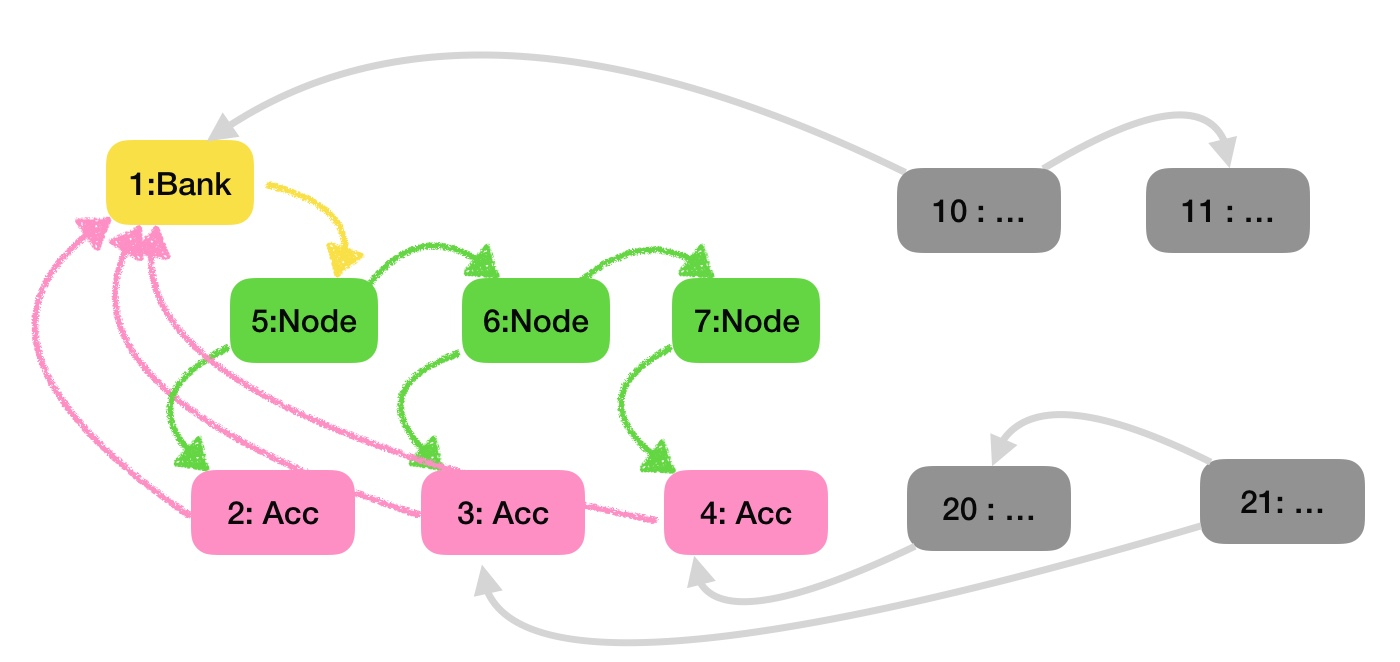
\includegraphics[width=10cm,height=4.5cm]{diagram1}
 \caption{Diagrammatic representation of some objects from  \prg{Bank}, \prg{Account} \etc  }
  \label{fig:Diagram}
  \end{figure}


\subsection{The Problem}

Now, we want to be able to give a formal meaning to things proposed in ~\cite{ELang}. eg that   

 
\begin{description}
\item[Pol\_2]
Only someone with the bank of a given currency can violate conservation of that currency.
 \item[Pol\_4]
No one can affect the balance of an account they don't have.
\end{description}

When we are executing lines 13 and 14 from above we are temporarily modifying the currency without having access to the \prg{Bank}. So, the states when executing the code from lines 13 and 14  should be considered ``invisible'', and ignored when we describe {\prg{Pol\_2}}. Similarly, when calling
function \prg{updateBalance} we do not necessarily have (directly) access to  the corresponding account,
so you could say that the function \prg{updateBalance} invalidates {\prg{Pol\_4}}.
Therefore, we see that a specification should be able express which states it considers  ``invisible''.


\noindent  
{\em What we did so far:} 
As of July, we ignored this issue, and were expressing these policies as below:

 
\begin{definition}
\label{def:internal}
We define  the set of objects \prg{o}   internal to a bank  or an account  z,  as follows:

%  \noindent
%$\prg{Internal}(\prg{b})$ \ \  $\triangleq$ \ \
%$\{\ \prg{o}\ \mid\  \prg{b}:\prg{Bank}\ \ \wedge \ \ (\ \prg{o} = \prg{b}\ \ \vee\  \ \prg{o}:\prg{Account}\wedge \prg{o}.\prg{myBank}=\prg{b}$\\
%\strut \hspace{7.3cm} $\ \ \vee\ \ \ \exists k. \ \prg{b}.\prg{ledger}.\prg{next}^k = \prg{b})\ \ \ \ \}$
%
%$\prg{Internal}'(\prg{a})$ \ \  $\triangleq$ \ \
%$\{\ \prg{o}\ \mid\  \prg{a}:\prg{Account}\ \ \wedge \ \
% \prg{a}.\prg{myBank} :\prg{Bank}\ \wedge\  \prg{o}\in \prg{Internal}(\prg{b})\ \}$


$\prg{Internal}(\prg{z})$ \ \  $\triangleq$ \ \
$\left\{
  \begin{array}{ll}
     \{\ \prg{o}\ \ \mid\     \ \prg{o} = \prg{z}\ \ \vee\  \ \prg{o}:\prg{Account}\wedge \prg{o}.\prg{myBank}=\prg{z} \\
 \strut \hspace{0.96cm} \vee\ \ \ \exists k. \ \prg{z}.\prg{ledger}.\prg{next}^k = \prg{o} \ \ \ \ \} , 
  & \hbox{if \prg{z}:\prg{Bank}} \\
   \{\ \prg{o}\ \mid\   \
 \prg{z}.\prg{myBank} :\prg{Bank}\ \wedge\  \prg{o}\in \prg{Internal}(\prg{z})\ \ \},  
& \hbox{if \prg{z}:\prg{Account}}\\
\{ \ \}, & \hbox{otherwise}
  \end{array} 
\right.$
\end{definition}

Looking at the diagram from Fig. \ref{fig:Diagram}, the objects $\{ 1, 2, 3, 4, 5, 6, 7 \}$  are internal to $1$, and  also internal to $4$. The set of objects internal to $6$ is empty.
We can now look at the policies, and formalize  as follows:

\begin{definition}
Policy \Pol 2 promises that if \prg{b} was a \prg{Bank}, and its  \prg{currency} were to change, and 
the set of objects involved in that change was \prg{S}, then there is at least one object in \prg{S} which has access to \prg{b}, and which is not internal to \prg{b}. And similar for \Pol 4. Formally:


\label{def:internal}
  \Pol 2\ \  $\triangleq$ \ \
  $\forall \prg{b}.\forall \prg{S}.
  [ \ \  \prg{b}:
  \prg{Bank}\ \wedge\ \prg{this}\neq\prg{b}\ \wedge\ \ \Using{(\Future\Changes{\prg{b.currency}})}{\prg{S}} \ \ \ \ \longrightarrow \ \  $\\
   \strut $~ $ \ \ \ \hspace{.7in}  \hfill
 $\exists \prg{o}. \ [ \ \
  \prg{o}\in \prg{S}\   \wedge\  \CanAccess{\prg{o}}{\prg{b}}\ \wedge\     \prg{o}\notin\prg{Internal}(\prg{b})  \ \ ]\ \ ]$


 \vspace{.1cm}
% \noindent
    \Pol 4\ \  $\triangleq$\ \ $\forall \prg{a}.\forall \prg{S}.\ [ \ \  \prg{a}:\prg{Account}\   \wedge\   \prg{this}\neq\prg{a} \ \wedge\ \Using{(\Future\Changes{\prg{a.balance}})}{\prg{S}}\ \ \   \
    \longrightarrow$ \\
 $\strut \hspace{.7in} \hfill \exists \prg{o}.\ [\, \prg{o}\in \prg{S}\ \wedge \ \CanAccess{\prg{o}}{\prg{a}}\ \wedge  \ \prg{o} \notin\prg{Internal}(\prg{a}) \ ] \ \ \ \ ]$

\end{definition}
 
An example illustrating that the code from Fig. 1 does not satisfy \Pol 2 is when we called, say,
 \prg{2.deposit(3)}. This will eventually lead to the calls \prg{5.updateBalance(100)} and
 \prg{6.updateBalance(-100)}.  The set of objects involved in the   first call is $\{\ 5 \}$, which is an object that is internal to $1$. The  first call reduces the currency by $100$, and thus we have violated 
\Pol 2. However, the  second call
increases it by $100$, and thus net effect on \prg{currency} is none.  Therefore, we want to
express that for this policy all the states between the beginning of \prg{6.updateBalance(-100)} and its end are ``invisible''.


\footnote{Note that the requirements $\prg{this}\neq \prg{b}$ and $\prg{this}\neq \prg{a}$ are annoying, but at the moment I do not know how to avoid them. Consider this an orthogonal problem.}
 
 
% \paragraph{The problem}

  
  \section{Possible Solutions} 
  
 I see the following four alternatives
  
\subsection{Solution\_1: Postpone}
Just ignore the question for the time being


Advantage:  we do not solve too many problems together. Several examples from the contracts literature can be expressed withoutthese concerns (as many simple contracts do not have auxiliary objects).


Disadvantage: there is simple code from the object capabilities literature which does not adhere to policies.

\subsection{Solution\_2: Visible States from the Invariant Literature.}

Adapt the solutions that were developed in the invariants literature -- a survey can be 
found at \cite{DrossoFrancaMuellerSummers08}.
 
Advantage:  we would be adapting known technology.
Disadvantage:  it is a bit inflexible, and it
 requires some different-style tools than what we have so far.

\subsection{Solution\_3: Maximal Flexibility}


We add one more assertion-constructor, which says which are the states which it considers visible.

The assertion $\VisibleLit(A,B)$ says that $A$ holds in a semantics which only considers states whose  receiver is  in the set  described by $B$; all other states are "skipped". That is, we have a new operational semantics, which considers some part of execution as atomic. \footnote{Perhaps we need a stratified system, where the set description $B$ is not as expressive as $A$}.

Then, policy \Pol 2 would be
 
  \Pol 2\ \  $\triangleq$ \ \
  $\forall \prg{b}.\forall \prg{S}.
  [ \ \ \prg{b}:
  \prg{Bank} \ \ \ \rightarrow $\\
$ \strut \hspace{1.4in} \ \VisibleLit$ (   \\
$ \strut \hspace{1.7in}\ \Using{(\Future\Changes{\prg{b.currency}})}{\prg{S}} \ \ \ \longrightarrow \ \  $\\
 \strut $~ $ \ \ \ \hspace{2.0in}   
 $\exists \prg{o}. \ [ \ \
  \prg{o}\in \prg{S}\   \wedge\  \CanAccess{\prg{o}}{\prg{b}}\ \wedge\     \prg{o}\notin\prg{Internal}(\prg{b})  
\ \ ],$ \\
  $ \strut \hspace{1.7in} \ \prg{External(b})$ \ ) $ \ \ ]$

\noindent 
and where the external objects to \prg{o} is the complement of the internals.

 \noindent
$\prg{External}(\prg{z},\prg{o})$ \ \  $\triangleq$ \ \   $ \prg{o} \notin \prg{Internal}(\prg{z})$

Therefore, the assertion from above says, that for all banks, if we consider as visible only the states whose receiver is not internal to a bank \prg{b}, and if and the  \prg{currency} of \prg{b} changes
the set of objects involved in that change was \prg{S}, then there is at least one object in \prg{S} which has access to \prg{b}, and which is not internal to \prg{b}.

\vspace{.3in}
\noindent
Advantage:  flexible.
\\
Disadvantage:  it requires the satisfaction judgment to be a bit more complex, and have the form 
$\M, B, \sigma \models A$. But doable.

\noindent
We would define things as follows. First, define that a state $\sigma$ is visible for $B$:

\begin{itemize}
\item
$\M, \sigma \Vdash B$\ \ iff\ \ $ \sigma(\this)\in \interp{B}{\sigma,\M}$
\end{itemize}

Then, define the operational semantics, which records only the states that are visible for $B$:

\begin{itemize}
\item
$\M , \sigma \leadsto_B \sigma'$ \\  iff\\
  $\M, \sigma \Vdash B$, \ and\  $\M, \sigma \Vdash B$, \ and \\
    $\exists n\geq 0. \exists \sigma_1, ... \sigma_n.$\\  
    $[ \ \M, \sigma \leadsto \sigma_1\, \wedge\,  \M, \sigma_1 \leadsto \sigma_2  ... \wedge  \M, \sigma_n \leadsto \sigma' \ \wedge\ \,
      \M, \sigma_1 \not\Vdash B\, \wedge\ \M, \sigma_2 \not\Vdash B\,  ... \wedge\,  \ \M, \sigma_n \not\Vdash B\ ]$.
\end{itemize}



Finally, we define   satisfaction by cases as follows:
\begin{itemize}
\item
$\M, B, \sigma \models e$ \ \ iff \ \  $ \M, \sigma \Vdash B\ \wedge\  \interp{e}{\sigma} = true$
\item
$\M, B, \sigma \models \Changes{e} $  \ \ iff \ \  $\exists \sigma'.  [\ \sigma \leadsto_B^* \sigma' \ \wedge \ \interp{e}{\sigma}\neq \interp{e}{\sigma'}\ ]$
\item
$\M, B, \sigma \models  \VisibleLit(A,B')$   \ \ iff \ \    $\M, B\cap B', \sigma \models A $
\item
... etc ...
\end{itemize}


\subsection{Solution\_4: Reduced Flexibility}
 
Instead of making a general-purpose assertion-constructor, we expand the ones we have now, to say that a change, or a future effect is observed when considering a restricted set of visible states. So We will have:\\
  $\Changes {e,B}$ says that a change in $e$ is observed with visible states as described in $B$, and \\ $\Future {(A,B)}$ says that at some future point which is observable through visible states as described in $B$ the assertion $A$ will hold, and\\
$\Past {(A,B)}$ says that at some past point which was observable through visible states as described in $B$ the assertion $A$ held.

With these assertions, we describe \Pol 2 as follows
  
  \Pol 2\ \  $\triangleq$ \ \
  $\forall \prg{b}.\forall \prg{S}.
  [ \ \ \prg{b}:
  \prg{Bank} \ \ \wedge\ \ \Using{(\Future\Changes{\prg{b.currency},\prg{External(b)}})}{\prg{S}} \ \ \ \longrightarrow \ \  $\\
 \strut $~ $ \ \ \ \hspace{2.0in}   
 $\exists \prg{o}. \ [ \ \
  \prg{o}\in \prg{S}\   \wedge\  \CanAccess{\prg{o}}{\prg{b}}\ \wedge\     \prg{o}\notin\prg{Internal}(\prg{b})  
\ \ ] \ \ ]$

\vspace{.3in}
\noindent
Advantage:  easier to make the semantics.
\\
Disadvantage:  ad hoc, and a bit repetitive.
 If we combine many things observed under the same visible states, then it
will become ugly, eg  something like $\Changes{\prg{e},\prg{B}} \ \rightarrow \Changes{\prg{e'},\prg{B}}$ is less natural than $\VisibleLit(\Changes{\prg{e}} \ \rightarrow \Changes{\prg{e'}},\prg{B})$

We would define it as follows

\begin{itemize}
\item
$\M,  \sigma \models e$ \ \ iff \ \  $\interp{e}{\sigma} = true$ // ie as in July version
\item
$\M, \sigma \models \Changes{e,B} $  \ \ iff \ \  $\exists \sigma'.  [\ \sigma \leadsto_B^* \sigma' \ \wedge \ \interp{e}{\sigma}\neq \interp{e}{\sigma'}\ ]$
\item
$\M, \sigma \models  \Future {(A,B)}$   \ \ iff \ \     $\exists \sigma'.  [\ \sigma \leadsto_B^* \sigma'\  \wedge\ \M, \sigma \models A\ ]$
\item
... etc ...
\end{itemize}

\subsection{Solution\_5: Encode it}

I think we do not need new assertion-constructors, but can encode as follows:
\vspace{.1in}

\noindent 
  \Pol 2\ \  $\triangleq$ \ \
  $\forall \prg{b}.\forall \prg{S}.\forall \prg{v}:$\\
  $\strut \hspace{.3in} [ \ \ \prg{b}:
  \prg{Bank} \ \  \wedge\ \ \prg{b.balance}=\prg{v}  \ \  \wedge\ \ \this\notin\prg{Internal}(\prg{b})$\\
 $\strut \hspace{0.999in}  \wedge \ \  \Using{\Future{(\prg{b.currency}\neq \prg{v} \ \  \wedge\ \ \this\notin\prg{Internal}(\prg{b})\ \ )}}{\prg{S}} \ \ \  $
 \\
  $\strut  \hspace{.4in}  \longrightarrow $\\  
  $\strut  \hspace{.4in}   \exists \prg{o}. \ [ \ \
  \prg{o}\in \prg{S}\   \wedge\  \CanAccess{\prg{o}}{\prg{b}}\ \wedge\     \prg{o}\notin\prg{Internal}(\prg{b})  
\ \ ] \ \ ]$

The above says that if  the current state is external to the bank \prg{b} (ie  the current receiver is not internal to   \prg{b}), and the current balance is \prg{v}, and  if in some future state  external to \prg{b}  the balance of \prg{b} is no longer \prg{v}, then the set of objects used in effecting this change contains at least one object \prg{o} external to \prg{b} which has direct access to \prg{b}.

\vspace{.3in}
\noindent
Advantage:  we do not need any new concepts. Also, we no longer use the concept of $\Changes{\_}$. A bit verbose?
\\
Disadvantage:  is not as expressive as the previous two solutions, as it allows me to talk about any two consecutive external states, while the previous two solutions allowed me tot capture the nearest extrernal successor state. But I think it does the job for the examples we have considered so far. 


\section{Syntax}

What should the assertion-constructors look like? Should they be prefix when unary and infix when binary?
Should we use keywords rather than symbols, eg ${\bf future} \,A$ rather than  $\Future A$? And
$A\, {\bf observing}\, B$ rather than $\VisibleLit(A,B)$? I think that syntax is secondary, but perhaps it affects which of the
alternatives we 
(the design team) consider as 
easier to understand.

\section*{Bibliography}
 \bibliographystyle{acm} %{plain}
 \bibliography{Case}



\end{document}

